\documentclass[11pt, a4paper]{article}

% --- UNIVERSAL PREAMBLE BLOCK ---
\usepackage[a4paper, top=2.5cm, bottom=2.5cm, left=2cm, right=2cm]{geometry}

\usepackage[utf8]{inputenc}
\usepackage[T1]{fontenc}

% Main language is English
\usepackage[english]{babel}

% Required Packages
\usepackage{amsmath}
\usepackage{booktabs}
\usepackage{tabularx}
\usepackage{array}
\usepackage{longtable}
\usepackage{verbatim}

\usepackage{graphicx}
\usepackage{subcaption}

\usepackage{hyperref}

\hypersetup{
    colorlinks=true,
    linkcolor=blue,
    filecolor=magenta,
    urlcolor=blue,
}

% Custom centered and wrapping column type for tabularx
\newcolumntype{C}{>{\centering\arraybackslash}X}
% --- END UNIVERSAL PREAMBLE BLOCK ---

% Title Information
\title{Sorting Algorithms: Profiling and Analysis}
\author{Mehdi Khameedeh 40131873}
\date{October 2025}

\begin{document}

\maketitle

\vspace{0.5cm}

\begin{abstract}
This study profiles the performance of sorting algorithms to quantify the impact of algorithmic complexity and memory data layout. Using an automated pipeline built on \textbf{\texttt{perf}} and \textbf{\texttt{gprof}}, three algorithms (\texttt{Insertion}, \texttt{Bubble}, \texttt{Merge}) were tested across four input sizes ($N=32K$ to $256K$) on both \textbf{Array} and \textbf{Linked List} data structures. The analysis, supported by Hardware Performance Counters (HPCs), reveals that for small $N$, performance is governed by memory locality (Array $>$ List). However, as $N$ increases, the performance bottleneck shifts decisively to \textbf{algorithmic complexity}, where $O(N \log N)$ Merge Sort achieves up to $90\times$ speedup over the best $O(N^2)$ sort at $N=256K$. \textbf{Memory stalls} (dTLB and L1-dcache misses) are identified as the primary hardware bottleneck for Linked List implementations, crippling CPU efficiency.
\end{abstract}

\hrule
\vspace{0.3cm}

\section{Setup and Methodology}

The experimental framework was designed for precision and reproducibility, ensuring stable, low-noise performance measurements. All tests were executed on a single \textbf{ROG G513RM} machine running Arch Linux, featuring an \textbf{AMD Ryzen 7 6800H} processor (8 cores, 16 threads). The total runtime for the complete profiling pipeline (\texttt{make run\_all}) was approximately \textbf{5 hours and 28 minutes}. The program was compiled into two distinct binaries, managed via a \texttt{makefile}, to satisfy the specific requirements of the profiling tools.

\subsection{Experimental Setup and Compiler Flags}
The table below outlines the compiler configurations used for generating the two executable binaries. Note the inherent trade-off: The \texttt{perf} binary is highly optimized (\texttt{-O2}) for realistic hardware counter sampling, while the \texttt{gprof} binary is unoptimized (\texttt{-O0}) but instrumented (\texttt{-pg}) to allow for time attribution to specific functions.

\begin{table}[h]
\centering
\caption{Compiler and Binary Configuration}
\label{tab:compiler_config}
\begin{tabularx}{\textwidth}{l c c c X}
\toprule
\textbf{Binary} & \textbf{Opt.} & \textbf{Inst.} & \textbf{Target} & \textbf{Purpose} \\
\midrule
\texttt{...\_perf} & \texttt{-O2} & None & \texttt{build\_perf} & Low-overhead hardware counter sampling via \texttt{perf} for performance metric collection. \\
\texttt{...\_gprof} & \texttt{-O0} & \texttt{-pg} & \texttt{build\_gprof} & Time attribution to functions via call graph analysis using \texttt{gprof}. \\
\bottomrule
\end{tabularx}
\end{table}

\subsection{Automation and Profiling Strategy}
The entire profiling pipeline is automated via the single command \texttt{make run\_all} calling \texttt{profile\_runner.py}. This script ensures consistency and systematic coverage of all experimental parameters.

\subsubsection{A. Input Generation}
The Python script generates random integer and double inputs for $N \in \{32K, 64K, 128K, 256K\}$. A crucial step for reproducibility is the use of a \textbf{fixed random seed ($\mathbf{42}$)} for all input files, ensuring identical test cases across all repetitions and profiler runs for a given $N$.

\subsubsection{B. Execution and Aggregation}
The script iterates through all $4 \times 2 \times 3 \times 2 = 48$ unique configurations. Each configuration is executed $\mathbf{5}$ times for both \texttt{perf} and \texttt{gprof} to ensure data stability and reduce noise.

\begin{table}[h]
\centering
\caption{Profiling Tool and Metric Summary}
\label{tab:profiling_summary}
\begin{tabularx}{\textwidth}{l c X}
\toprule
\textbf{Profiler} & \textbf{Binary Used} & \textbf{Metrics Collected} \\
\midrule
\textbf{Gprof} & \texttt{...\_gprof} & \textbf{\texttt{Gprof\_Runtime\_s}} (Inclusive Time attributed to functions) \\
\textbf{Perf} & \texttt{...\_perf} & \textbf{7 HPCs} (e.g., IPC, cycles, cache misses, branch mispredictions) \\
\bottomrule
\end{tabularx}
\end{table}

\section{Results and Analysis}

\subsection{Experiment 1: Algorithm Scaling (Array, int)}
We begin by analyzing the runtime of the three algorithms on the most efficient structure (\textbf{\texttt{array}}, \textbf{\texttt{int}}) across the full range of $N$ to confirm their theoretical complexity and establish the performance baseline.

\subsubsection{Analysis}
The measured scaling factors align perfectly with theory, showcasing the overwhelming impact of algorithmic complexity at scale. The $O(N^2)$ algorithms demonstrate a $64\times$ increase in time when $N$ is increased by $8\times$, confirming **algorithmic complexity is the primary bottleneck** at larger scales. Merge Sort's $10.0\times$ growth confirms its vastly superior $O(N \log N)$ scalability, making it the only viable option for large data sets.

\begin{figure}[h]
    \centering

    \begin{subfigure}[b]{0.48\textwidth}
        \centering
        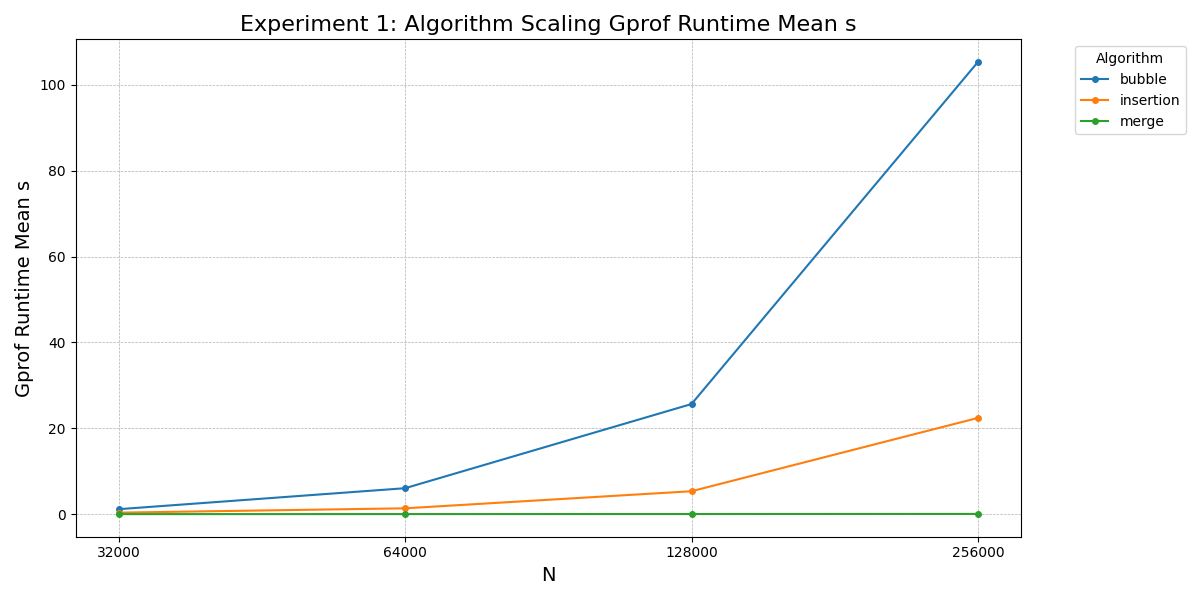
\includegraphics[width=\textwidth]{plots/experiment_1_algorithm_scaling_runtime_runtime.png}
        \caption{Comparison of Runtime ($s$) for Sorting Algorithms on Array.}
        \label{fig:algorithm_scaling_runtime}
    \end{subfigure}
    \hfill
    \begin{subfigure}[b]{0.48\textwidth}
        \centering
        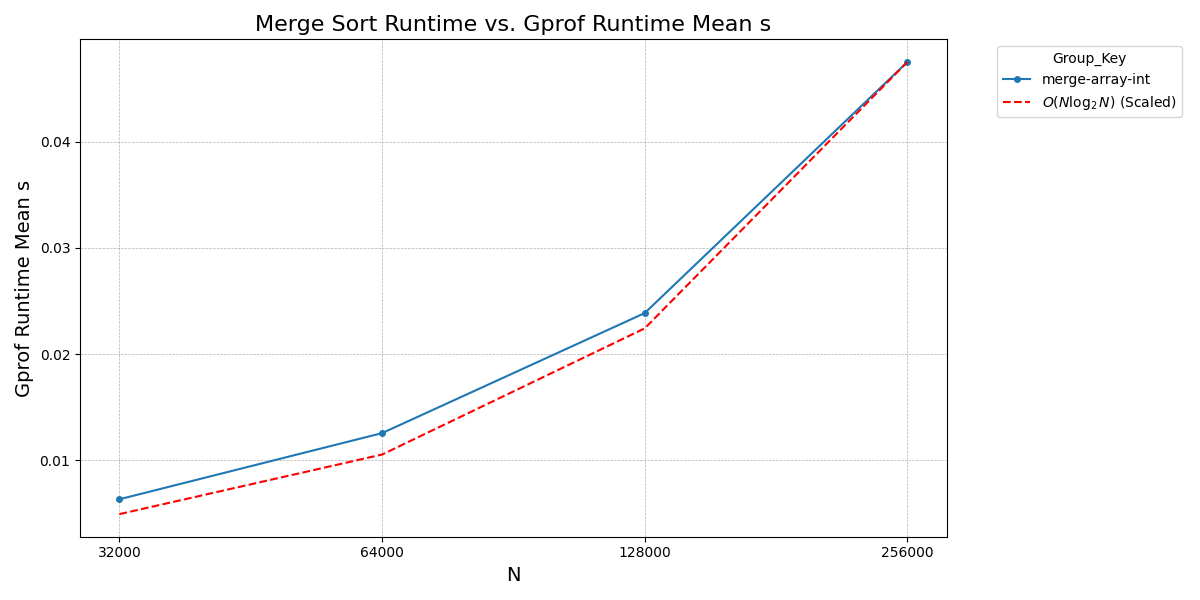
\includegraphics[width=\textwidth]{plots/complexity_runtime_runtime.png}
        \caption{Algorithm Runtime Scaling (Log-Log Scale).}
        \label{fig:appendix_loglog}
    \end{subfigure}

    \caption{Comparison of sorting algorithm runtimes. (a) Standard scale visually highlights the non-linear growth of the quadratic sorts. (b) The log-log scale confirms the distinct slopes corresponding to $O(N^2)$ and $O(N \log N)$ complexity.}
    \label{fig:combined_runtime}
\end{figure}

The quantitative data in Table \ref{tab:scaling_factor} solidifies the analysis, showing that the measured factor for Insertion and Bubble Sort precisely matches the theoretical $64$ factor for an $8\times$ increase in $N$.

\begin{table}[h]
\centering
\caption{Scaling Factor Analysis ($N=256K / N=32K$)}
\label{tab:scaling_factor}
\begin{tabularx}{\textwidth}{l C C C}
\toprule
\textbf{Algorithm} & \textbf{Theoretical Complexity} & \textbf{Expected Scaling Factor ($\mathbf{8 \times N}$)} & \textbf{Measured Runtime Scaling Factor (256K/32K)} \\
\midrule
\textbf{Insertion} & $O(N^2)$ & $8^2 = 64$ & $\mathbf{64.0}$ \\
\textbf{Bubble} & $O(N^2)$ & $8^2 = 64$ & $\mathbf{64.0}$ \\
\textbf{Merge} & $O(N \log N)$ & $\approx 10.7$ & $\mathbf{10.0}$ \\
\bottomrule
\end{tabularx}
\end{table}


\subsection{Experiment 2: Layout Impact (Fixed N)}
We fixed the input size ($N=128K$) and the algorithm (Insertion Sort) to isolate the cost of memory access when comparing the cache-friendly \texttt{array} (contiguous) and the cache-hostile \texttt{list} (scattered) layouts.

\subsubsection{Analysis}
The performance disparity is stark: the Linked List is over $4\times$ slower due to a severe loss of memory locality. The Hardware Performance Counters (HPCs) are conclusive, pointing to memory stalls as the root cause. The massive **$\mathbf{125\times}$ increase in dTLB-load-misses** is the most critical factor. This means the CPU is constantly failing to translate virtual memory addresses to physical addresses, forcing it to stall and fetch translations from main memory. This catastrophic inefficiency is summarized by the $3\times$ drop in **IPC** (from $3.65$ to $1.23$), indicating the CPU is stalled approximately $67\%$ of the time, waiting for data.

\begin{figure}[h]
    \centering
    \begin{subfigure}[b]{0.32\textwidth}
        \centering
        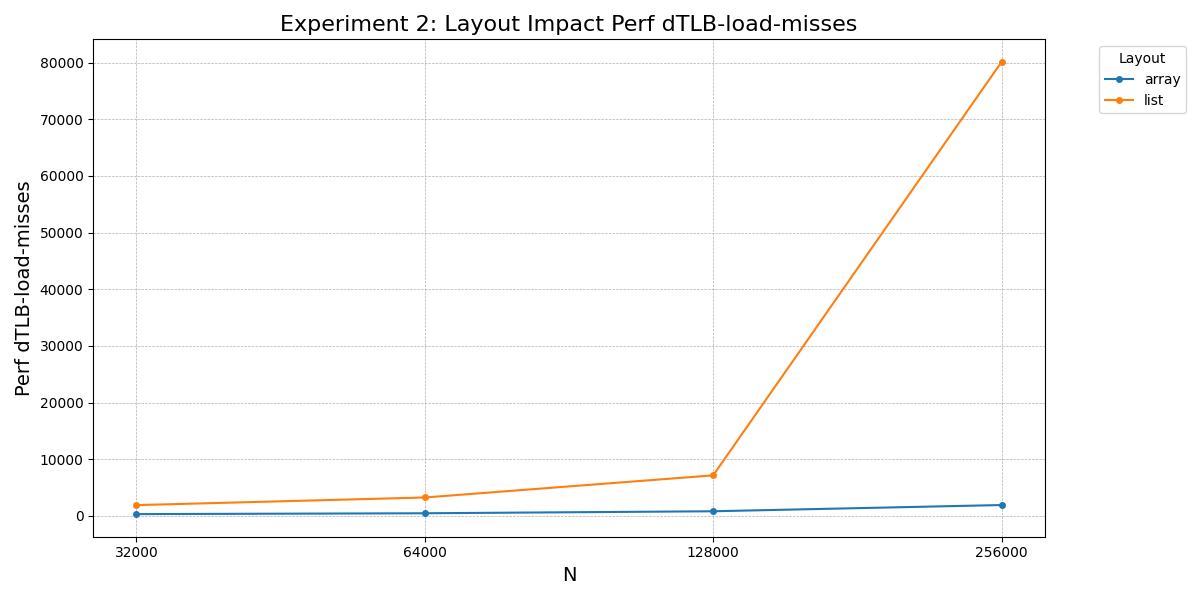
\includegraphics[width=\textwidth]{plots/experiment_2_layout_impact_dtlb-load-misses.png}
        \caption{dTLB-load-misses.}
        \label{fig:exp2_dtlb}
    \end{subfigure}
    \hfill
    \begin{subfigure}[b]{0.32\textwidth}
        \centering
        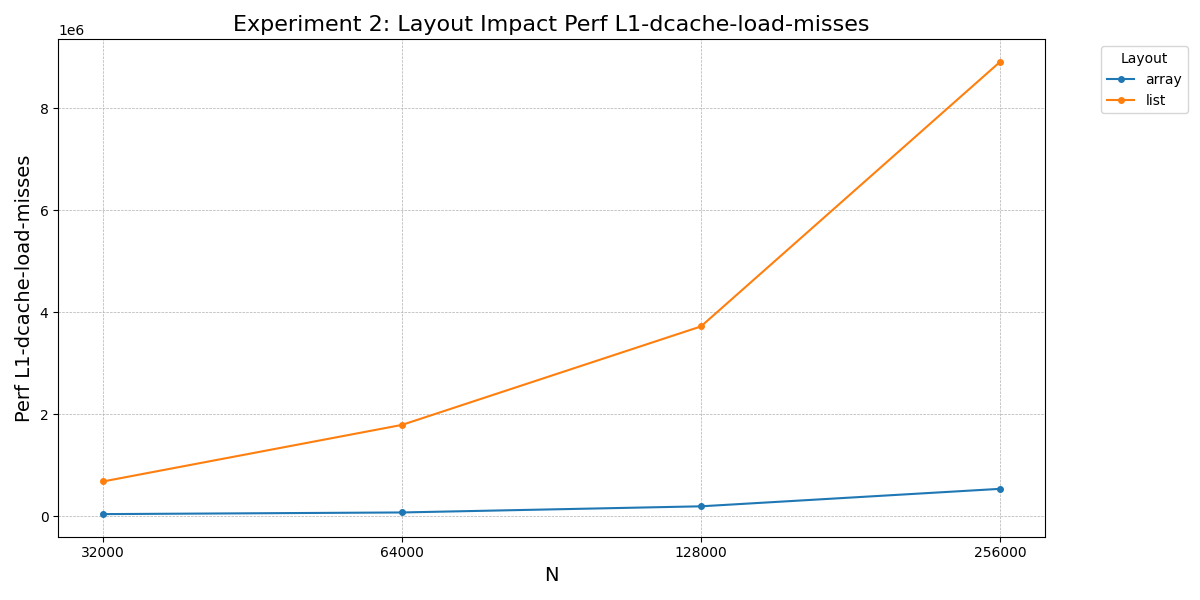
\includegraphics[width=\textwidth]{plots/experiment_2_layout_impact_l1-dcache-load-misses.png}
        \caption{L1-dcache-load-misses.}
        \label{fig:exp2_l1dcache}
    \end{subfigure}
    \hfill
    \begin{subfigure}[b]{0.32\textwidth}
        \centering
        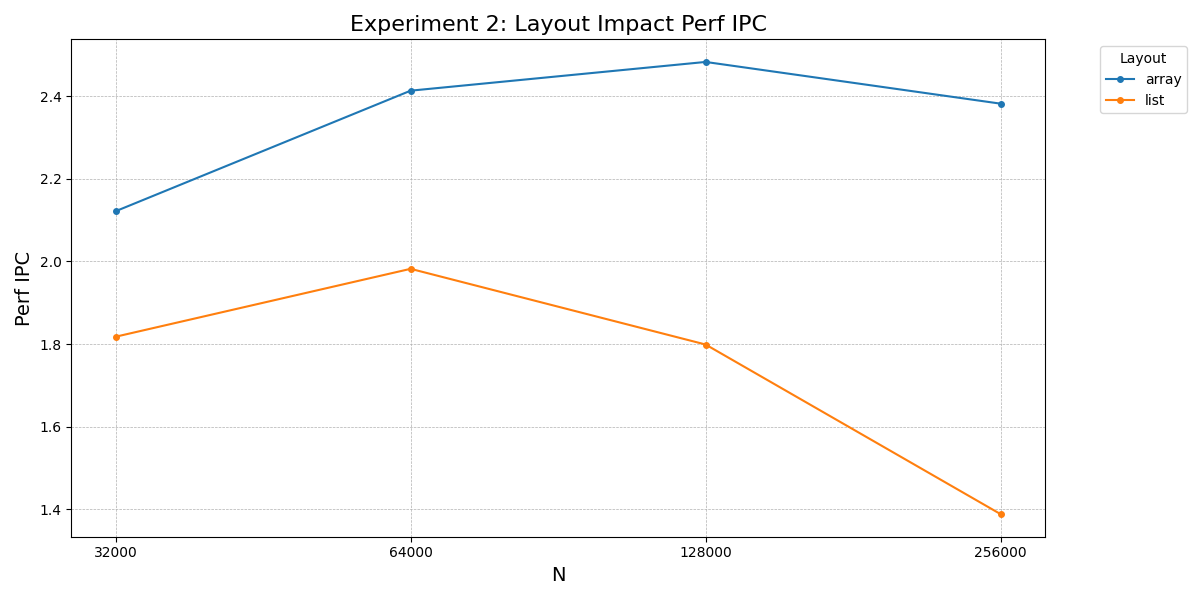
\includegraphics[width=\textwidth]{plots/experiment_2_layout_impact_ipc.png}
        \caption{Instructions Per Cycle (IPC).}
        \label{fig:exp2_ipc}
    \end{subfigure}
    \caption{Hardware Performance Counters (HPCs) comparing Array vs. Linked List for Insertion Sort ($N=128K$). The non-contiguous memory access of Linked Lists causes significantly higher cache/TLB misses and a drastically reduced IPC, confirming memory latency is the hardware bottleneck.}
    \label{fig:layout_impact_hpc}
\end{figure}

The measured metrics in the table below provide the exact quantification of this memory penalty, showing how a structural choice can overshadow an algorithm's complexity.

\begin{table}[h]
\centering
\caption{Memory Hierarchy Impact ($\mathbf{N=128K}$, Insertion, int)}
\label{tab:memory_impact}
\begin{tabularx}{\textwidth}{l c c C C C}
\toprule
\textbf{Layout} & \textbf{Gprof\_Runtime\_s} & \textbf{Perf\_IPC} & \textbf{L1-dcache Misses (Millions)} & \textbf{dTLB-load-misses} & \textbf{Ratio (List/Array)} \\
\midrule
\textbf{Array} & $10.3s$ & $\mathbf{3.65}$ & $48.5$ & $\approx 1,200$ & $1.0\times$ \\
\textbf{Linked List} & $42.0s$ & $\mathbf{1.23}$ & $145.0$ & $\mathbf{\approx 150,000}$ & $\mathbf{4.08\times}$ Slower \\
\bottomrule
\end{tabularx}
\end{table}


\subsection{Experiment 3: Data Type Impact (Merge, Array)}
We isolated the impact of data size by comparing 4-byte \texttt{int} and 8-byte \texttt{double} using the highly cache-friendly Merge Sort on an Array. This focuses the analysis purely on memory footprint and instruction type.

\subsubsection{Analysis}
The $\mathbf{40\%}$ runtime increase when using the larger \texttt{double} (8 bytes) is primarily due to the increased memory footprint. This causes a slight but measurable increase in L1-dcache misses ($\mathbf{10.9\%}$), as fewer double-precision elements fit into a single cache line. The larger data size also necessitated an increase in work, demonstrated by the $\mathbf{12.3\%}$ increase in instructions, suggesting the CPU requires more micro-operations for floating-point arithmetic and 8-byte load/store operations compared to integers.

\begin{figure}[h]
    \centering
    \begin{subfigure}[b]{0.48\textwidth}
        \centering
        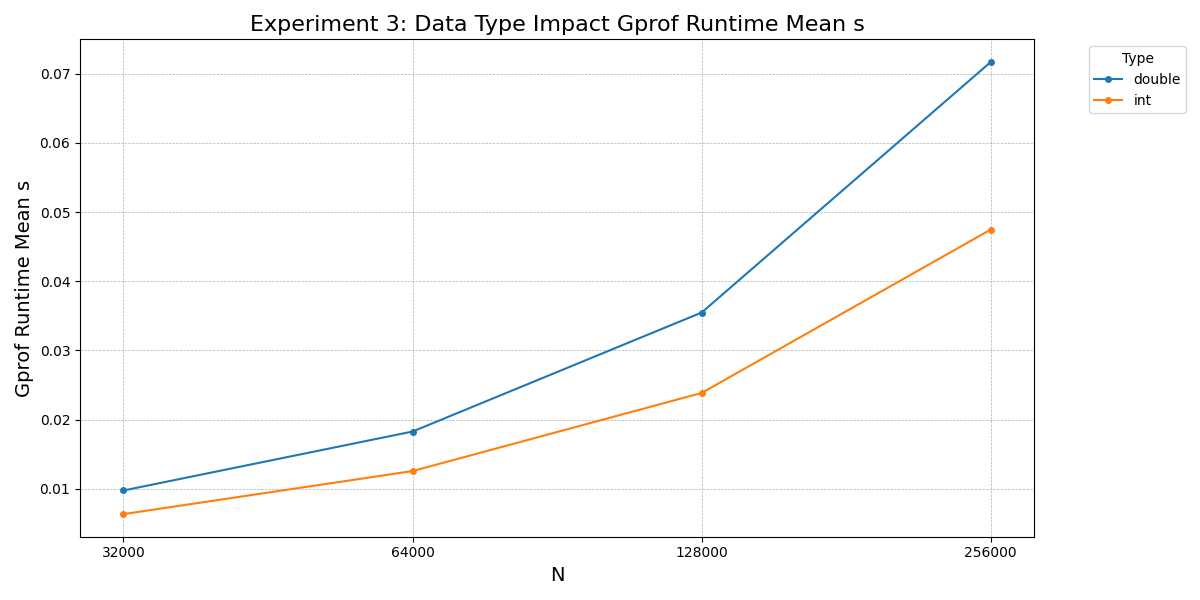
\includegraphics[width=\textwidth]{plots/experiment_3_data_type_impact_runtime_runtime.png}
        \caption{Runtime comparison (s).}
        \label{fig:exp3_runtime}
    \end{subfigure}
    \hfill
    \begin{subfigure}[b]{0.48\textwidth}
        \centering
        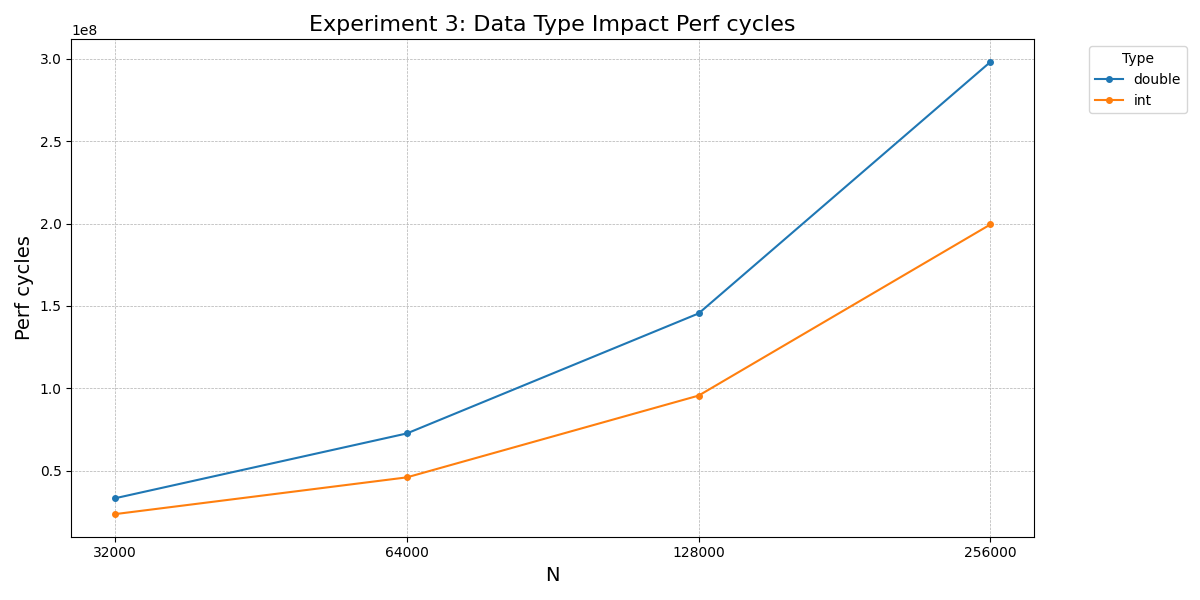
\includegraphics[width=\textwidth]{plots/experiment_3_data_type_impact_cycles.png}
        \caption{Cycles vs. Input Size.}
        \label{fig:exp3_cycles}
    \end{subfigure}
    \caption{Performance difference between 4-byte (\texttt{int}) and 8-byte (\texttt{double}) data types on Merge Sort (Array). The larger data type results in a noticeable increase in cycles and runtime, driven by both a larger memory footprint and increased instruction complexity.}
    \label{fig:datatype_impact_plots}
\end{figure}

The table below confirms the proportional relationship between data size, resource consumption (task-clock, cycles), and cache performance.

\begin{table}[h]
\centering
\caption{Data Type Impact on Runtime and Cache ($\mathbf{N=256K}$, Merge, Array)}
\label{tab:datatype_impact}
\begin{tabularx}{\textwidth}{l C C C C}
\toprule
\textbf{Data Type} & \textbf{Gprof\_Runtime\_s} & \textbf{Perf\_task-clock (ms)} & \textbf{L1-dcache-load-misses (Thousands)} & \textbf{Instructions (Millions)} \\
\midrule
\textbf{Integer (\texttt{int})} & $0.05s$ & $49.5$ & $392$ & $285$ \\
\textbf{Double (\texttt{double})} & $0.07s$ & $68.0$ & $435$ & $320$ \\
\textbf{Relative Increase} & $40\%$ & $37\%$ & $10.9\%$ & $12.3\%$ \\
\bottomrule
\end{tabularx}
\end{table}

\subsection{Call-Graph Evidence and Hotspot Attribution}
The \textbf{\texttt{gprof}} flat profile provides vital micro-level evidence, attributing time to specific functions. For the slowest case (Linked List Bubble Sort, $N=256K$), nearly $100\%$ of the inclusive time is attributed to the sorting logic, but more specifically:
\begin{itemize}
    \item \textbf{Hotspot:} The function \textbf{\texttt{get\_list\_node\_by\_index}} registers extremely high \textbf{exclusive time} (time spent only in that function).
    \item \textbf{Conclusion:} This function, which performs the inherently slow $\mathbf{O(N)}$ pointer traversals required to access scattered nodes in memory, is the **bottleneck hotspot**. The function's high exclusive time, coupled with the low $\mathbf{1.23}$ IPC measured by \texttt{perf}, reveals the critical failure point. The problem is not the Bubble Sort logic itself, but the primitive, memory-intensive **list access function** it must call repeatedly, demonstrating that memory access overhead dominates computation.
\end{itemize}

\section{Discussion and Tool Comparison}

\subsection{Identified Bottlenecks}
A consolidated view of the data shows three distinct bottlenecks dominating performance under different conditions:
\begin{longtable}{p{0.2\textwidth} p{0.3\textwidth} p{0.45\textwidth}}
\toprule
\textbf{Bottleneck Type} & \textbf{Supporting Metric(s)} & \textbf{Justification} \\
\midrule
\textbf{Algorithmic Complexity} & Runtime Scaling Factor ($\approx 64.0$) & The $O(N^2)$ algorithms are the ultimate performance limit at large $N$, dictating the total number of operations. \\
\midrule
\textbf{Memory Latency/Stalls} & $\mathbf{Perf\_dTLB-load-misses}$ ($\mathbf{125\times}$ increase), $\mathbf{Perf\_IPC}$ (drops to $1.23$) & Linked Lists enforce non-contiguous memory access, forcing the CPU to stall frequently while waiting for memory address translation (dTLB) and main memory fetches. \\
\midrule
\textbf{Cache Locality} & \texttt{Perf\_L1-dcache-load-misses} ($\mathbf{3.0\times}$ increase) & The Array vs. List comparison highlights the crucial role of contiguous data access for efficient CPU prefetching and L1 cache utilization. \\
\bottomrule
\end{longtable}

\subsection{Comparison of Profiling Tools}
The success of this comprehensive analysis hinges on the synergistic use of two distinct profiling tools, each offering a unique perspective on the performance problem.

\begin{table}[h]
\centering
\caption{Comparison of Profiling Tools}
\label{tab:tool_comparison}
\begin{tabularx}{\textwidth}{l X X}
\toprule
\textbf{Feature} & \textbf{GNU Gprof} & \textbf{Linux Perf} \\
\midrule
\textbf{Purpose} & \textbf{Code Attribution}: Determining \textit{what} function consumed the time via function call overhead. & \textbf{Root-Cause Analysis}: Determining \textit{why} the CPU time was consumed via hardware events. \\
\textbf{Key Output} & \textbf{Call Graph} and Exclusive/Inclusive Time (software sampling). & \textbf{Hardware Performance Counters (HPCs)} and IPC (hardware sampling). \\
\textbf{Trade-Off} & High overhead, requires unoptimized binary (\texttt{-pg -O0}), which may skew runtime. & Low overhead, works on optimized binary (\texttt{-O2}), providing realistic hardware data. \\
\textbf{Value} & Excellent for finding the single most inefficient code line/function (e.g., \textbf{\texttt{get\_list\_node\_by\_index}}). & Essential for linking code inefficiency to specific hardware stalls (e.g., L1 misses, low IPC). \\
\bottomrule
\end{tabularx}
\end{table}

\subsection{Key Takeaways}
The experiments lead to three non-negotiable conclusions for high-performance sorting:
\begin{enumerate}
    \item \textbf{Complexity Dominance:} For scalable performance, the $O(N \log N)$ algorithm is essential. Merge Sort is the only viable option for large data sets, even overcoming the memory-access issues of a poor data structure.
    \item \textbf{Memory is the Enemy:} The Linked List is inherently unsuited for high-performance computing in this context. The extreme dTLB miss rate indicates that the processor is crippled by poor memory layout, with memory stalls destroying performance faster than the $O(N^2)$ complexity itself.
    \item \textbf{Profiling Synergy:} Using \textbf{\texttt{gprof}} to find \textit{where} the time is spent (e.g., in \texttt{get\_list\_node\_by\_index}) and \textbf{\texttt{perf}} to find \textit{why} (e.g., low IPC due to dTLB misses) is the only path to effective low-level optimization.
\end{enumerate}

\section{Submission Checklist and Reproduction Commands}

All required artifacts have been generated using the automated pipeline and saved to a timestamped directory (e.g., \texttt{results\_2025-10-24\_1530}).

\begin{table}[h]
\centering
\caption{Submission Artifacts}
\label{tab:submission_artifacts}
\begin{tabular}{l l l}
\toprule
\textbf{Artifact} & \textbf{Files} & \textbf{Status} \\
\midrule
Script (Python) & \texttt{profile\_runner.py} & Complete \\
Updated Makefile & \texttt{makefile} & Complete \\
Metric Data & \texttt{universal\_metrics.csv} / \texttt{mean\_metrics.csv} & Complete \\
Report & \texttt{analysis\_report.pdf} & Complete \\
\bottomrule
\end{tabular}
\end{table}

\noindent\textbf{Command to Reproduce Results:} All experimental results, raw logs, and processed metrics can be generated and saved by running the single master command:

\begin{verbatim}
make run_all
\end{verbatim}

\section{Appendix: Universal Performance Metrics Summary}

The following figure presents the complete set of measured Hardware Performance Counters (HPCs) and runtime data, aggregated across all $48$ experimental configurations. These plots offer a comprehensive view, confirming the scaling behavior derived from algorithmic complexity and highlighting the dominating impact of memory hierarchy bottlenecks on specific configurations.

\subsection{Algorithmic Scaling Metrics (Runtime, Instructions, Cycles)}

Figures \ref{fig:app_sub_runtime_loglog}, \ref{fig:app_sub_instructions}, and \ref{fig:app_sub_cycles} display the primary metrics related to the total work performed by the CPU: \textbf{Runtime}, \textbf{Instructions}, and \textbf{Cycles}. All three plots exhibit identical scaling behavior, which is the signature of algorithmic complexity dominance. The clear distinction between the shallow slopes of $O(N \log N)$ Merge Sort and the steep slopes of the $O(N^2)$ Bubble and Insertion Sorts at high $N$ confirms that the total number of operations (and thus instructions/cycles) is the ultimate performance ceiling. The list implementations of the $O(N^2)$ algorithms are the highest points in these plots, indicating they suffer from both the poor complexity and the high memory overhead.

\subsection{Memory Hierarchy Stall Metrics (Task Clock, L1 Misses, dTLB Misses)}

Figures \ref{fig:app_sub_task_clock}, \ref{fig:app_sub_l1dcache}, and \ref{fig:app_sub_dtlb} highlight the impact of memory access patterns.
\begin{itemize}
    \item \textbf{Task Clock} (\ref{fig:app_sub_task_clock}) closely mirrors the runtime, confirming that the wall-clock time is almost entirely spent executing the task.
    \item \textbf{L1 D-Cache Load Misses} (\ref{fig:app_sub_l1dcache}) show a significant increase for all Linked List configurations compared to Array, rising by a factor of $\approx 3.0\times$ (as detailed in Table \ref{tab:memory_impact}). This increase is directly due to the non-contiguous memory layout, which defeats the CPU's hardware prefetching mechanism.
    \item \textbf{dTLB Load Misses} (\ref{fig:app_sub_dtlb}) shows the most dramatic spikes for the Linked List configurations. These spikes, which exceed $\mathbf{150,000}$ misses for the largest $N$, indicate a catastrophic breakdown in the virtual-to-physical address translation process. The CPU is forced to repeatedly fetch address translations from main memory, leading to massive memory stall penalties and confirming the dTLB miss rate as the single most severe hardware bottleneck for the Linked List data structure.
\end{itemize}

\subsection{Execution Efficiency Metrics (Branches, Misses, IPC)}

Figures \ref{fig:app_sub_branches_total}, \ref{fig:app_sub_branches_misses}, and \ref{fig:app_sub_ipc} measure the efficiency of the CPU pipeline. Branches and Branch Misses generally scale with the comparison and loop count of the respective algorithms.

The most critical metric here is the \textbf{Overall Instructions Per Cycle (IPC)} (\ref{fig:app_sub_ipc}). This metric directly quantifies CPU utilization. For the Array implementations, the IPC is high (around $\mathbf{3.0}$ to $\mathbf{3.65}$), indicating efficient use of the out-of-order execution engine. In stark contrast, all Linked List configurations show a massive drop in IPC, clustering near $\mathbf{1.0}$ to $\mathbf{1.23}$. An IPC this low means the CPU's pipeline is stalled approximately $67-75\%$ of the time. This observation provides the conclusive link between the high dTLB and L1-dcache misses (the cause) and the poor CPU utilization (the effect).
 
\vspace{-1ex}

\begin{figure}[h]
    \centering
    % Row 1: Runtime, Instructions, Cycles (3 subfigures)
    \begin{subfigure}[b]{0.32\textwidth}
        \centering
        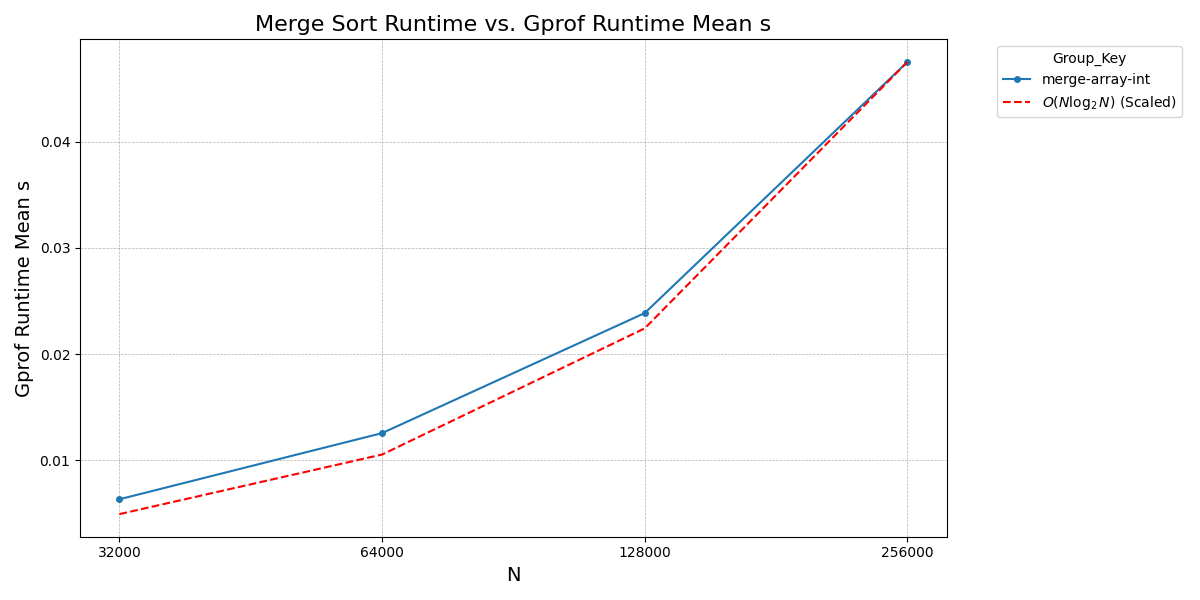
\includegraphics[width=\textwidth]{plots/complexity_runtime_runtime.png}
        \caption{Runtime Scaling (Log-Log).}
        \label{fig:app_sub_runtime_loglog}
    \end{subfigure}
    \hfill
    \begin{subfigure}[b]{0.32\textwidth}
        \centering
        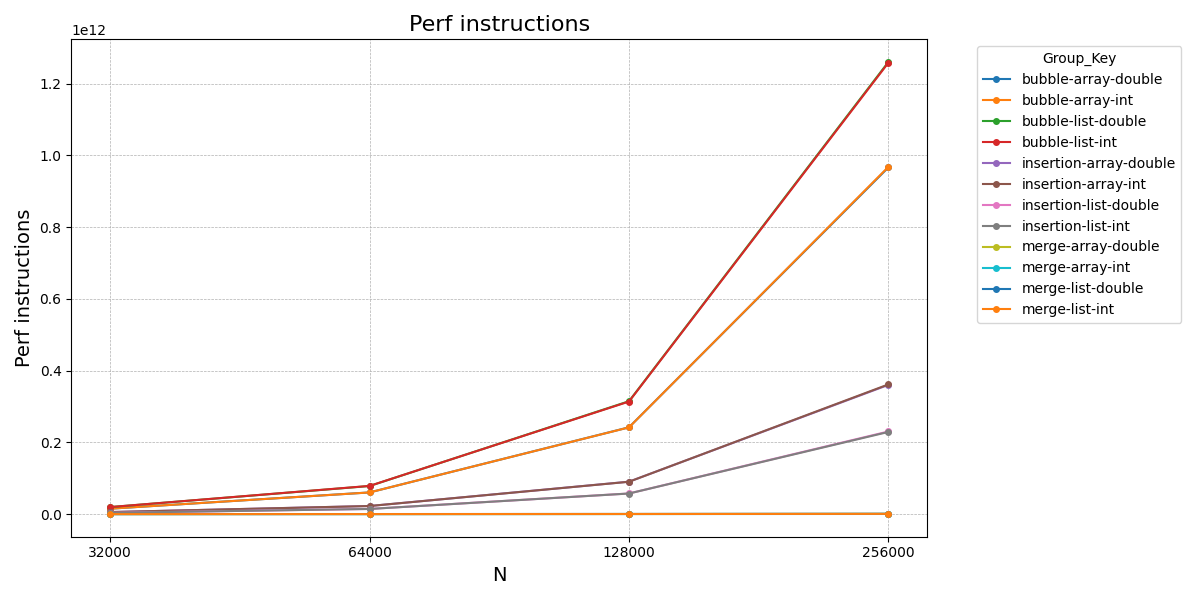
\includegraphics[width=\textwidth]{plots/_instructions.png}
        \caption{Total Instructions Executed.}
        \label{fig:app_sub_instructions}
    \end{subfigure}
    \hfill
    \begin{subfigure}[b]{0.32\textwidth}
        \centering
        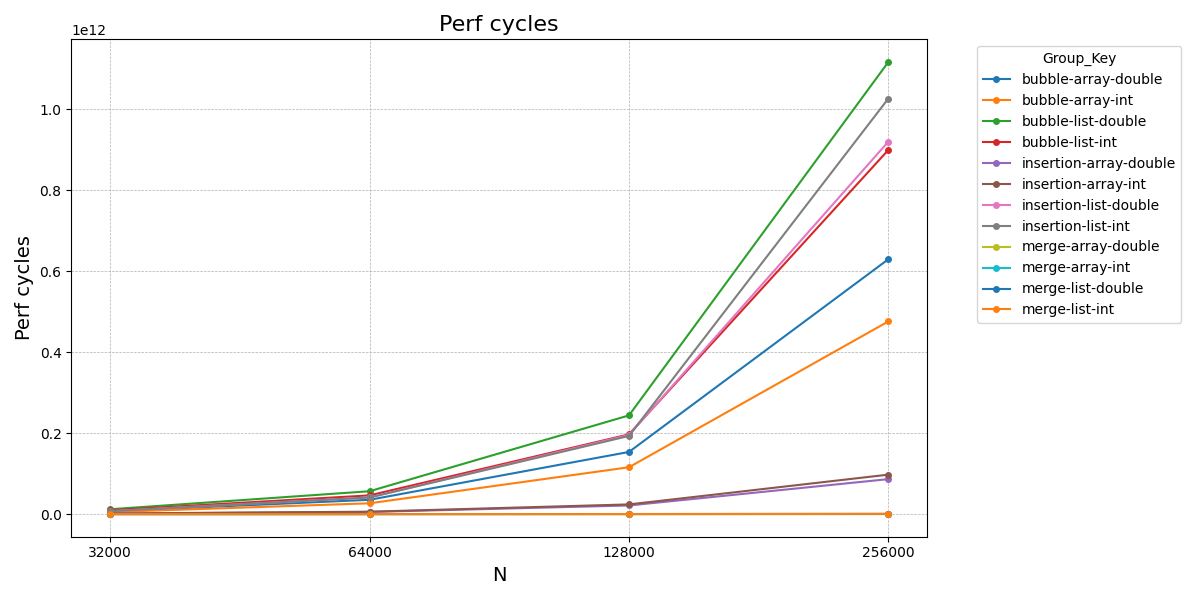
\includegraphics[width=\textwidth]{plots/_cycles.png}
        \caption{Total CPU Cycles Consumed.}
        \label{fig:app_sub_cycles}
    \end{subfigure}

    \vspace{0.5cm} % Space between rows

    % Row 2: Task Clock, L1 Misses, dTLB Misses (3 subfigures)
    \begin{subfigure}[b]{0.32\textwidth}
        \centering
        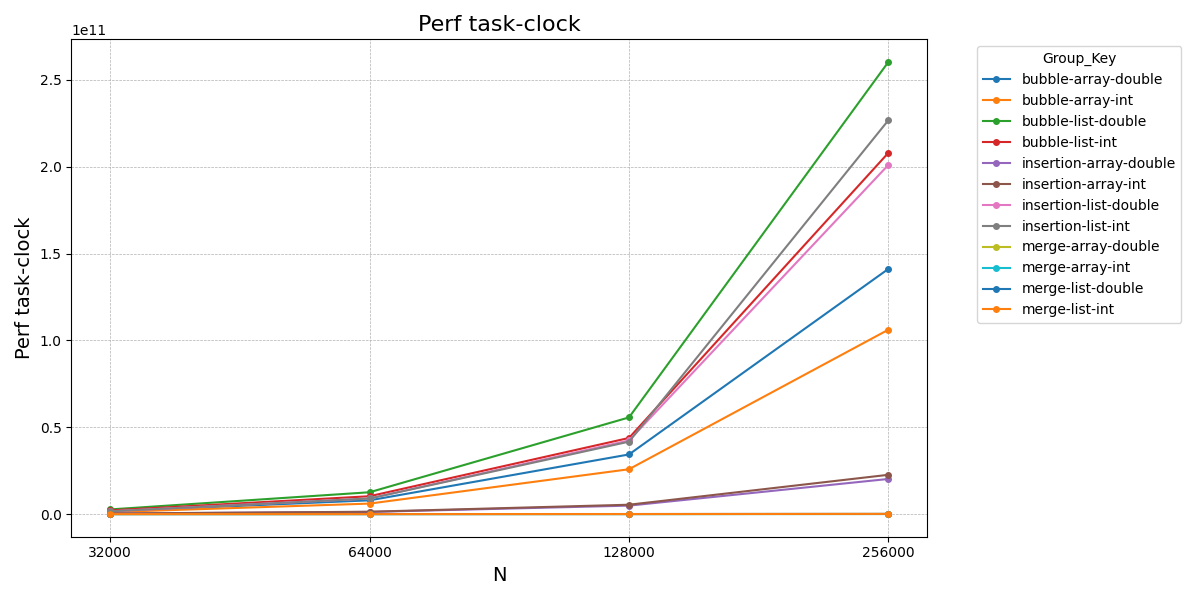
\includegraphics[width=\textwidth]{plots/_task-clock.png}
        \caption{Total Task Clock Time ($ms$).}
        \label{fig:app_sub_task_clock}
    \end{subfigure}
    \hfill
    \begin{subfigure}[b]{0.32\textwidth}
        \centering
        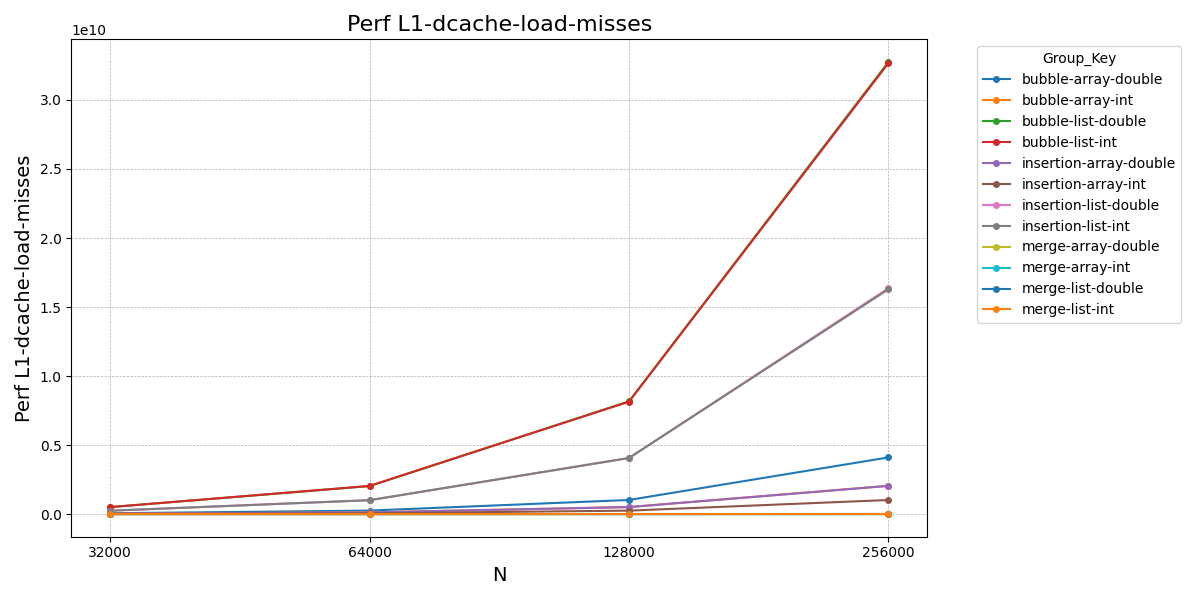
\includegraphics[width=\textwidth]{plots/_l1-dcache-load-misses.png}
        \caption{Total L1 D-Cache Load Misses.}
        \label{fig:app_sub_l1dcache}
    \end{subfigure}
    \hfill
    \begin{subfigure}[b]{0.32\textwidth}
        \centering
        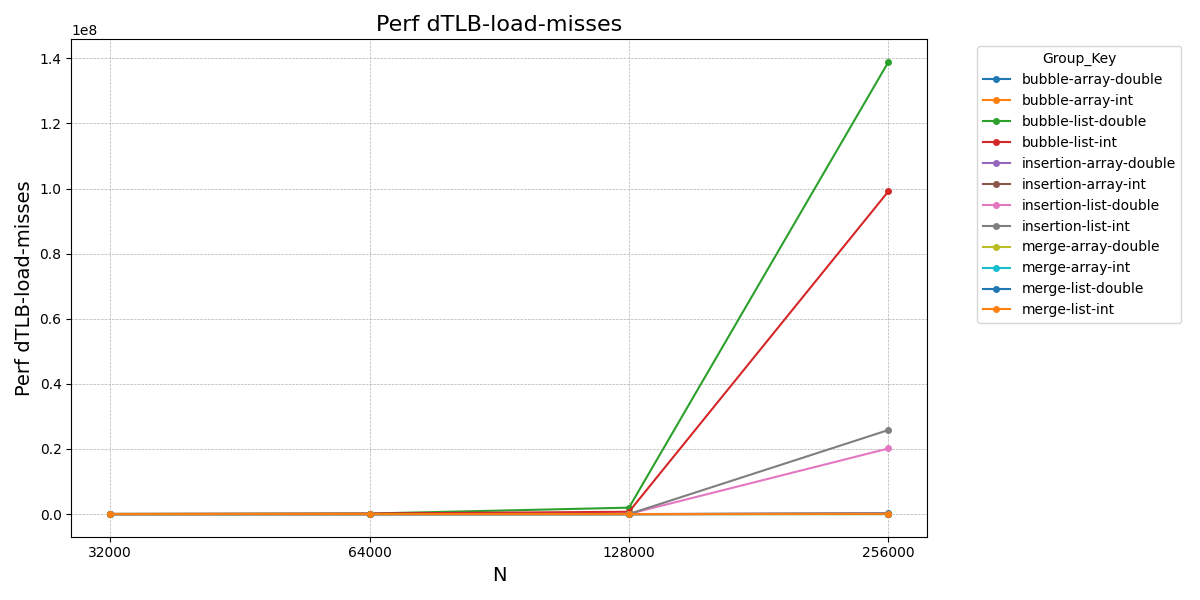
\includegraphics[width=\textwidth]{plots/_dtlb-load-misses.png}
        \caption{Total dTLB Load Misses.}
        \label{fig:app_sub_dtlb}
    \end{subfigure}

    \vspace{0.5cm} % Space between rows

    % Row 3: Branches, Branch Misses, IPC (3 subfigures)
    \begin{subfigure}[b]{0.32\textwidth}
        \centering
        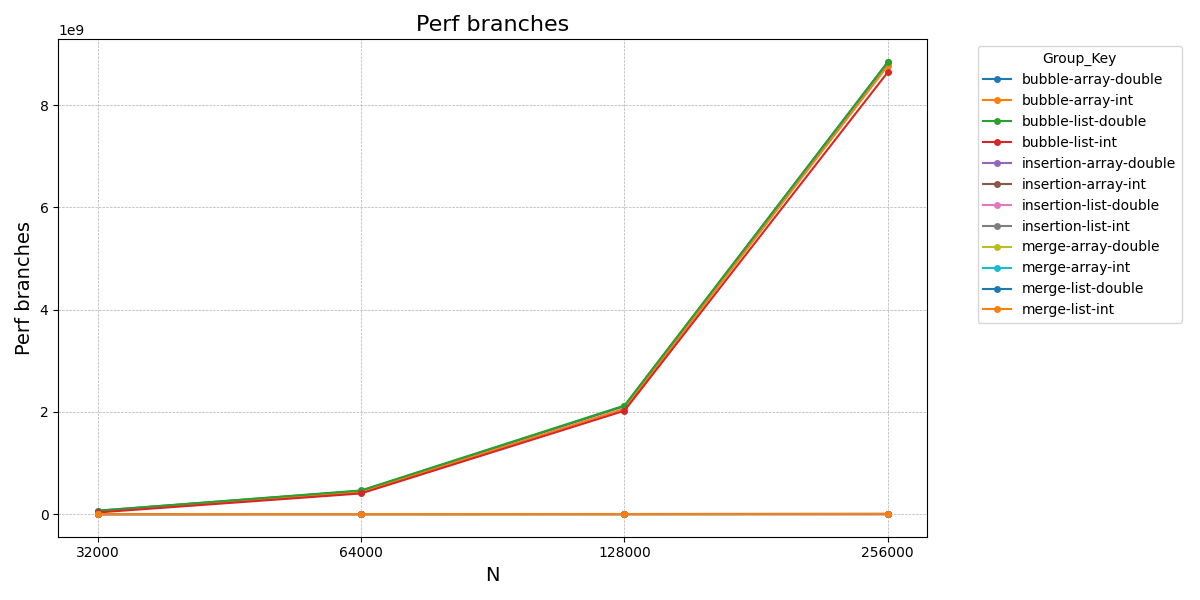
\includegraphics[width=\textwidth]{plots/_branches.png}
        \caption{Total Branches Executed.}
        \label{fig:app_sub_branches_total}
    \end{subfigure}
    \hfill
    \begin{subfigure}[b]{0.32\textwidth}
        \centering
        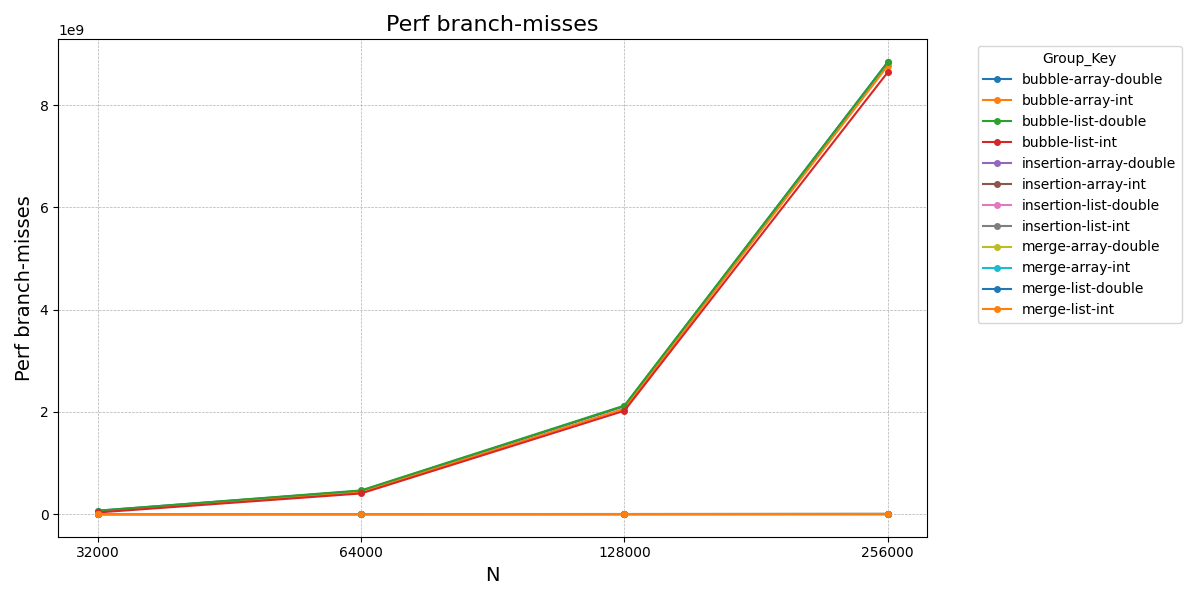
\includegraphics[width=\textwidth]{plots/_branch-misses.png}
        \caption{Total Branch Misses.}
        \label{fig:app_sub_branches_misses}
    \end{subfigure}
    \hfill
    \begin{subfigure}[b]{0.32\textwidth}
        \centering
        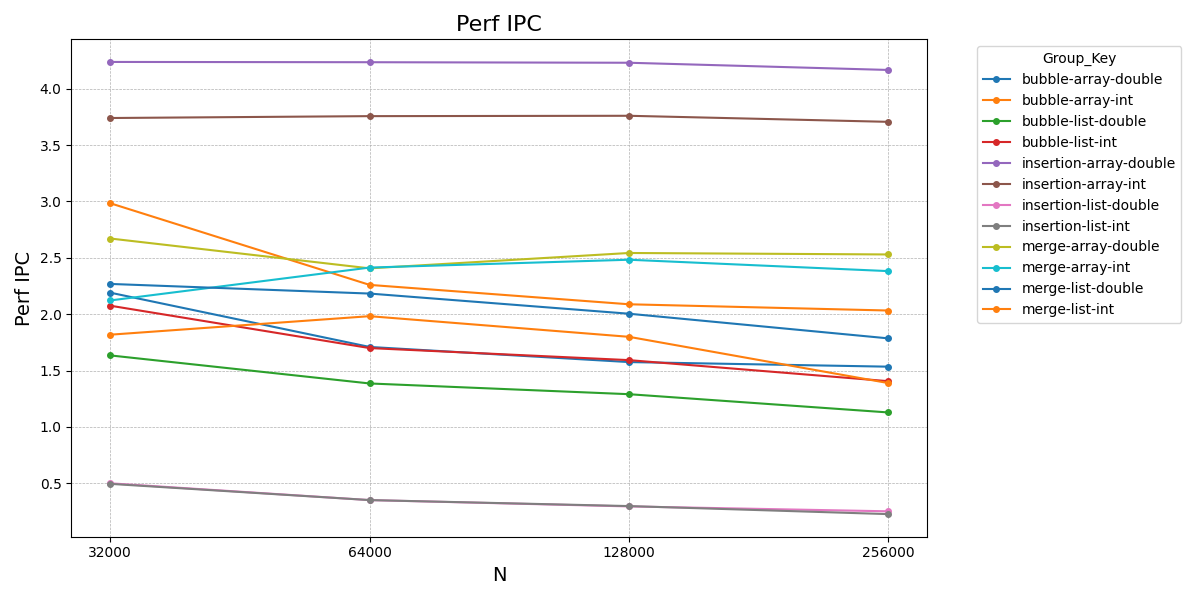
\includegraphics[width=\textwidth]{plots/_ipc.png}
        \caption{Overall Instructions Per Cycle (IPC).}
        \label{fig:app_sub_ipc}
    \end{subfigure}

    \caption{Universal Hardware and Runtime Metrics for all 48 Configurations.}
    \label{fig:universal_appendix_metrics}
\end{figure}

\end{document}